\documentclass[runningheads]{llncs}
\usepackage{graphicx}
\usepackage[utf8]{inputenc}
\usepackage{fancyhdr}
\usepackage{hyperref}
\usepackage{listings}
\usepackage{xcolor}
\usepackage{float}

\definecolor{codegreen}{rgb}{0,0.6,0}
\definecolor{codegray}{rgb}{0.5,0.5,0.5}
\definecolor{codepurple}{rgb}{0.58,0,0.82}
\definecolor{backcolour}{rgb}{0.95,0.95,0.92}
\lstdefinestyle{mystyle}{
    backgroundcolor=\color{backcolour},   
    commentstyle=\color{codegreen},
    keywordstyle=\color{magenta},
    numberstyle=\tiny\color{codegray},
    stringstyle=\color{codepurple},
    basicstyle=\ttfamily\footnotesize,
    breakatwhitespace=false,         
    breaklines=true,                 
    captionpos=b,                    
    keepspaces=true,                 
    numbers=left,                    
    numbersep=5pt,                  
    showspaces=false,                
    showstringspaces=false,
    showtabs=false,                  
    tabsize=2
}
\lstset{style=mystyle}
\pagestyle{fancy}
\fancyhf{}
\fancyhf{}
\rhead{ESPE}
\lhead{Universidad de las Fuerzas Armadas}
\rfoot{\thepage}
\renewenvironment{abstract}
{\quotation\small\noindent\rule{\linewidth}{.5pt}\par\smallskip
{\centering\bfseries\abstractname\par}\medskip}
{\par\noindent\rule{\linewidth}{.5pt}\endquotation}
\graphicspath{{../images/}}

\title{UPS Inteligente Utilizando Grafos}
\author{Alexander Guacán\orcidID{L00412289}}
\authorrunning{Universidad de las Fuerzas Armadas}
\institute{Universidad de las Fuerzas Armadas\\
\email{adguacan@espe.edu.ec}}

\begin{document}

    \maketitle

    \begin{abstract}
        % \textbf{Este documento sirve como modelo y guía para su informe. Puede reemplazar los encabezados y el cuerpo del texto con su contenido. Sin embargo, antes de comenzar a escribir, le recomendamos que considere detenidamente las instrucciones de este documento. El resumen describe en palabras concisas lo que hace, por qué lo hace (no necesariamente en este orden) y el resultado principal.}

        % El resumen debe ser autónomo y legible para una persona en el área general. Escriba un breve resumen de su proyecto o producto software, el cual se utiliza para ayudar al lector a determinar rápidamente el propósito de su reporte. Escribir únicamente un párrafo. Se recomienda incluir en el resumen al menos 100 palabras, pero no más de 200.
        El presente documento ha diseñado un programa que simula el funcionamiento de un Uninterruptable Power Supply (UPS), que a su vez se adaptó a un determinado escenario empleando el uso de grafos. Se analizó y creo dos algoritmos de búsqueda que determina el camino más corto a recorrer por un grafo desde un punto a otro. El escenario planteado es un cyber, el UPS tuvo la tarea de conocer el camino más corto por el circuito hasta un determinado dispositivo, para preservar su duración de encendido cuando el UPS usa su batería interna para suministrar energía eléctrica. Los resultados fueron los esperados pero queda en duda que algoritmo creado es el más óptimo o recomendado a utilizar en el escenario planteado.
        
    \end{abstract}

    %%%%%%%%%%%%%%%%%%%%%%%%%%%%%%%%%%%%%%%%%%%%%%%%%%%%%%%%%%%%%%%%%
    %%                        INTRODUCCIÓN                         %%
    %%%%%%%%%%%%%%%%%%%%%%%%%%%%%%%%%%%%%%%%%%%%%%%%%%%%%%%%%%%%%%%%%
    \section{Introducción}
        % La introducción es diferente del resumen; debería elaborar más sobre el contexto del trabajo y otros aspectos. Generalmente, puede repetir algunos de los puntos principales también en la introducción, pero amplíe y use palabras diferentes. Esta sección establece el propósito y los objetivos del escrito. 

        % La introducción generalmente describe el alcance del documento y ofrece una breve explicación del documento. También puede explicar ciertos elementos que son importantes en su proyecto si las explicaciones no forman parte del texto principal. Los lectores pueden tener una idea sobre el siguiente texto antes de empezar a leerlo. Para poder llegar a cumplir con lo antes mencionado, es importante presentar esta introducción de la manera más simple y directa posible. Escriba párrafos concisos y evite hacer listas o enumerar.  El número de párrafos que debe tener la introducción es de 3 a 4, lo cuales deben contener al menos 4 oraciones. 

        % Para evitar el \emph{plagio} y demostrar que ha entendido el tema de estudio, es fundamental parafrasear correctamente las ideas del autor. No copie y pegue partes del artículo, ni siquiera una o dos frases. La mejor manera de hacer esto es dejar el artículo a un lado y escribir su propia comprensión de los puntos clave del autor.

        Un UPS, por su traducción al español, es un Sistema de Alimentación Initerrumpida. Este dispositivo permite suministrar de energía eléctrica por un tiempo definido, cuando el flujo normal falla. Los fallos pueden darse cuando se va la luz o un cortocircuito, o cuando existe una sobrecarga en la energía eléctrica suministrada por el tomacorriente de la pared. Ahí es donde interviene el UPS, el cual se encarga de bloquear este mal flujo de corriente de energía eléctrica y suministrar su propia fuente de alimentación dado por una batería interna \cite{ups_definicion}.

        Por otra parte, un grafo es una estructura de datos que está representada a través del enlace de nodos, estos enlaces son conocidos como aristas. Cada nodo almacena cualquier tipo de información, y los datos de las aristas que posee \cite{grafo_definicion}. Por su parte, la teoría de grafos se encarga de estudiar el comportamiento y relación de estos últimos, como parte de una rama de las matemáticas aplicada en ciencias de la computación \cite{teoria_grafos_definicion}. Sus aplicaciones varían desde, buscar una ruta de un punto a otro, ya sea la más larga o corta. También se pueden utilizar en el manejo de las redes sociales, ya que al conocer los diferentes enlaces con amigos y patrones de sitios web visitados por el usuario, el algoritmo puede brindar de información más acorde al cliente sobre lo que desea consumir.

        En este laboratorio mezclaremos ambos conceptos, el objetivo será generar un sistema inteligente que simule el funcionamiento de un UPS. Establecer un escenario de funcionamiento del UPS en el cual pueda gestionar, a través del uso de grafos, un uso adecuado de su principal característica que es brindar energía eléctrica temporal. Comprender algoritmos de búsqueda aplicado a los grafos que permitan determinar el camino más corto de un punto a otro. El escenario que se plantea para este proyecto es un cyber. El principal problema será determinar el camino más corto desde el UPS hasta un cierto dispositivo para suminstrar energía directa al mismo para que su duración de encendido se incremente.
        
        %%%%%%%%%%%%%%%%%%%%%%%%%%%%%%%%%%%%%%%%%%%%%%%%%%%%%%%%%%%%%%%%%
        %%                     Desarrollo                              %%
        %%%%%%%%%%%%%%%%%%%%%%%%%%%%%%%%%%%%%%%%%%%%%%%%%%%%%%%%%%%%%%%%%
    \section{Desarrollo}
        % El desarrollo o cuerpo del ensayo en sí está organizado en párrafos. Recuerde que cada párrafo se centra en una idea o aspecto de su tema, y debe contener al menos 4-5 oraciones para que pueda abordar esa idea correctamente.

        % Cada párrafo del cuerpo tiene tres secciones. Primero está la oración principal. Esto le permite al lector saber de qué va a tratar el párrafo y el punto principal que hará. Da el punto del párrafo de inmediato. A continuación, y más grande, están las oraciones de apoyo. Estos amplían la idea central, explicándola con más detalle, explorando lo que significa y, por supuesto, dando la evidencia y el argumento que la respalda. Aquí es donde utiliza su investigación para respaldar su argumento. Luego hay una oración final. Esto reafirma la idea en la oración principal, para recordarle al lector su punto principal~\cite{fest1959}.

        % En la sección cuerpo del ensayo usted puede incluir imágenes las cuales deben estar referencias en el texto de forma mandatoria (vea Figura~\ref{sample_image}).
        Para diseñar el proyecto, primero comenzaremos explicando cada parte que conforma el UPS. Puede observar en la Figura \ref{fig:ups_circuito}, de forma simplificada, cada uno de los componentes que conforman un UPS. Es necesario especificar que existen distintos tipos de UPS y cada uno con capacidades distinas, en esta ocasión las características con las que cuenta el UPS a modelar son que sus voltajes de entrada que vienen desde el tomacorriente deben fluctuar entre $ 100 V $ y $ 140 V $. Además su voltaje de salida debe ser de $ 120 V $, donde su batería recibe y otorga un voltaje de $ 12 V $ con una intensidad de $ 9 Ah $ (Amperio/hora).

        \begin{figure}[H]
            \centering
            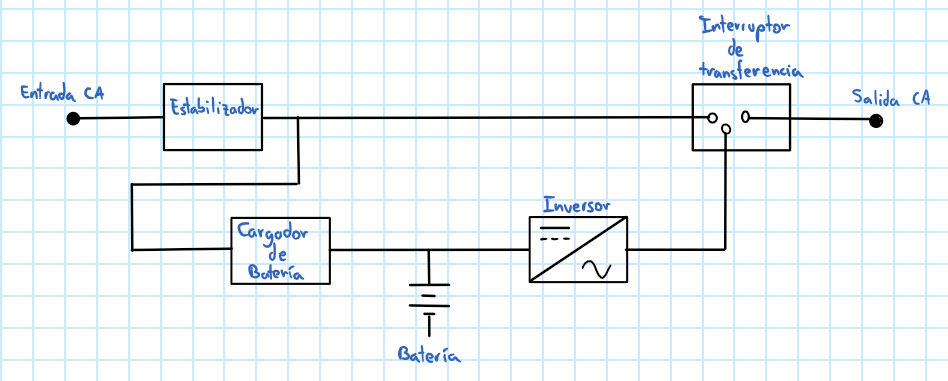
\includegraphics[width=\textwidth]{ups_circuito}
            \caption{Circuito eléctrico y componentes que conforman un UPS.}
            \label{fig:ups_circuito}
        \end{figure}
        
        El UPS cuenta con 3 modos o estados. El primero es el modo normal, observe Figura \ref{fig:ups_modo_normal}, aquí el voltaje esta dentro de los límites especificados en el anterior párrafo y la carga de la batería esta completa. Por lo que únicamente el estabilizador se encargará de regular el voltaje del tomacorriente a $ 120 V $ \cite{regulador_de_voltaje}. Se debe aclarar que el \emph{Interruptor de transferencia} unicamente sirve como puente entre los diferentes canales de corriente. En este modo se tomará la corriente desde el estabilizador, dado que no hay ningún problema con el voltaje leído desde el tomacorriente de pared \cite{ups_circuito}.
        
        \begin{figure}[H]
            \centering
            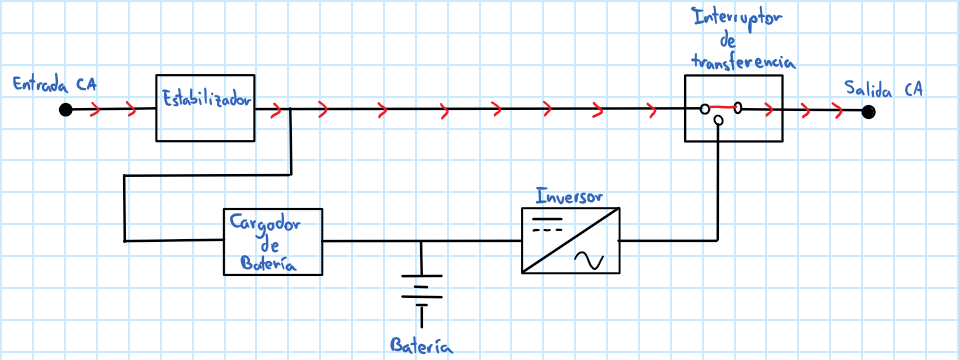
\includegraphics[width=\textwidth]{ups_modo_normal}
            \caption{Fluctuación de energía eléctrica en modo normal.}
            \label{fig:ups_modo_normal}
        \end{figure}

        El siguiente modo con el que cuenta el UPS es el modo normal pero sin carga. Este modo se refiere cuando el voltaje leído desde el tomacorriente cumple con los estándares estables, pero el porcentaje de la batería es menor al cien porciento. Para ello se comienza a cargar la batería a la vez que se suministra de forma normal energía eléctrica a los dispositivos. Observe que en la Figura \ref{fig:ups_modo_normal_carga} antes de que la corriente eléctrica del estabilizador llegue a la batería, debe pasar por su respectivo cargador. Este dispositivo se encarga de disminuir la corriente eléctrica de $ 120 V $ a $ 12 V $ que es lo necesario para cargar la batería \cite{cargador_de_bateria}.

        \begin{figure}[H]
            \centering
            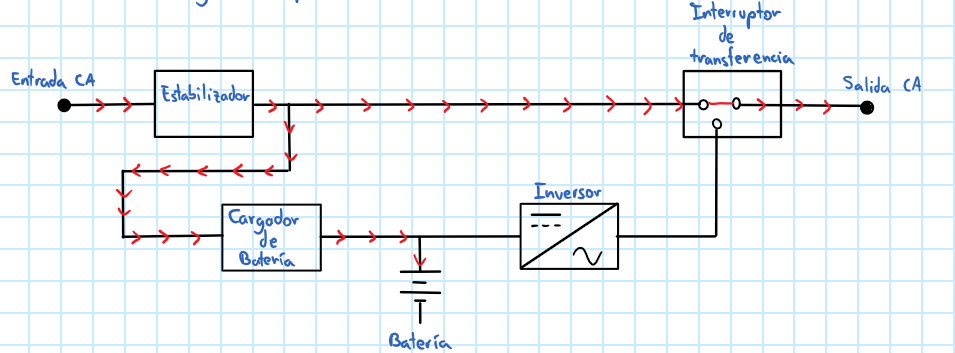
\includegraphics[width=\textwidth]{ups_modo_normal_carga}
            \caption{Fluctuación de energía eléctrica en modo normal pero con carga de batería incompleta.}
            \label{fig:ups_modo_normal_carga}
        \end{figure}
        
        Por último tenemos el modo inversor. En este modo el voltaje leído del tomacorriente se sale de los límites, existiendo un cortocircuito (menor a $ 100 V $) o una sobrecarga (mayor a $ 140 V $). Cuando se presenta uno de estos dos escenarios se comienza a utilizar la batería interna del UPS. Observe en la Figura \ref{fig:ups_modo_inversor} que ahora la energía eléctrica parte de la batería y pasa por el inversor, de ahí el nombre de dicho modo. El inversor se encarga de transformar la corriente directa que proporcia la batería en corriente alterna incrementada a $ 120 V $, necesarios para el correcto funcionamiento de los dispositivos \cite{inversor}. Es aquí cuando el estado de \emph{Interruptor de transferencia} cambia, haciendo un punte desde el estabilizador hacia la salida de corriente del UPS.
        
        \begin{figure}[H]
            \centering
            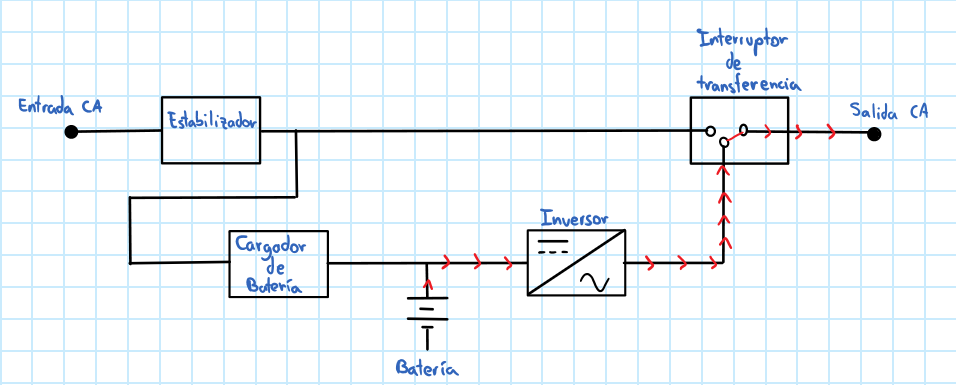
\includegraphics[width=\textwidth]{ups_modo_inversor}
            \caption{Fluctuación de energía eléctrica en modo inversor.}
            \label{fig:ups_modo_inversor}
        \end{figure}
        
        El grafo que simulará la distribución de los dispositivos en el cyber lo puede observar en la Figura \ref{fig:grafo_cyber}. Aquí podemos que el nodo cero representa al UPS y todos los demás nodos seran los dispositivos conectados a él. Observe también que un dispositivo puede ser otro "conector" pero en realidad lo que se refiere es que donde está conectado el dispositivo n, también existe otro conector junto como el de un cortapicos por el cual se puede ampliar la conexión de los dispositivos. Para hacerlo más flexible, permitiremos al usuario configurar el dispositivo que considere como principal.
        
        \begin{figure}[H]
            \centering
            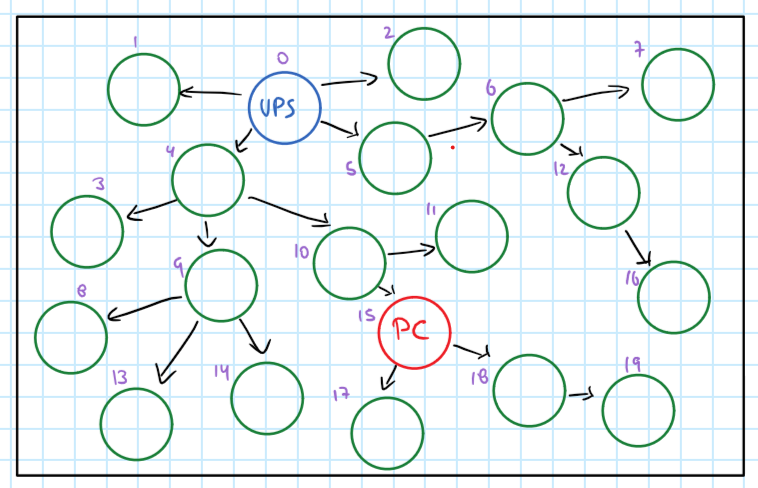
\includegraphics[width=\textwidth]{grafo_cyber}
            \caption{Distribución de los dispositivos de un cyber en forma de grafo.}
            \label{fig:grafo_cyber}
        \end{figure}
        
        Bien, el modelado de este problema respecto al UPS se ha optado por el patron observador. Este patrón trata de simular una suscripción a un canal, donde el canal será el componente observable y los suscriptores serán los observadores. Así pues en nuestro caso el UPS será el objeto observable y la pantalla donde se muestran las estadísticas será el observador. Puede observar en la Figura \ref{fig:uml_ups} que utilizamos interfaces para hacer una conexión entre ambos conceptos ya que de primeras no conocemos que tipo de elementos pueden observar o que componentes pueden ser observados. La interfaz \emph{Observable} cuenta con metodos para agregar, eliminar y notificar de cambios a los observadores, y por su parte la interfaz \emph{Observer} cuenta con un solo método el que se encargará de extraer la información de interés del objeto al cual observa.
        
        \begin{figure}[H]
            \centering
            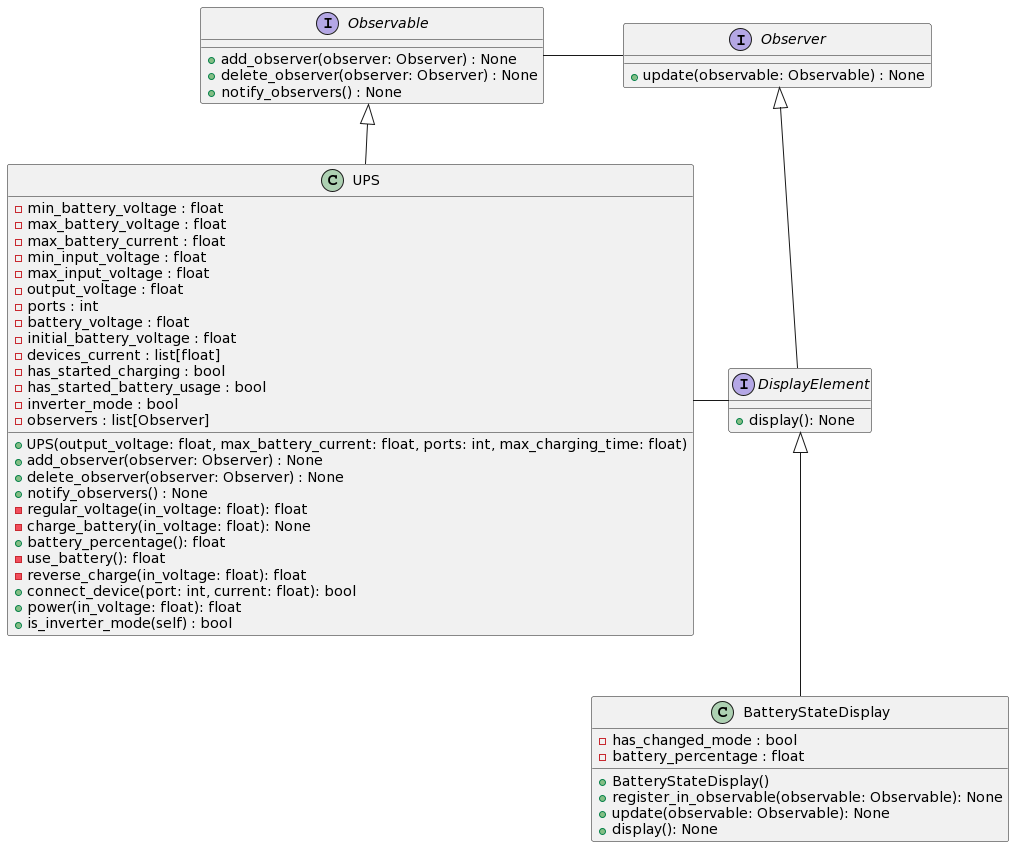
\includegraphics[width=\textwidth]{uml_ups}
            \caption{Diagrama de clases del UPS utilizando el patrón observador.}
            \label{fig:uml_ups}
        \end{figure}

        Antes de explicar el código recuerde que puede encontrar el código completo en \href{https://github.com/Alexander-Guacan/Proyecto_Unidad_3.git}{\textbf{GitHub}}. Asimismo puede observar una explicación más detallada de todo el proyecto en el siguiente \href{https://drive.google.com/file/d/1ghD_tkJbnypSG6MpYKVSDKDXMLQJQLaC/view?usp=sharing}{\textbf{Video}}. Para crear el grafo se ha empleado una lista de adyacencias, la cual consiste en que cada lista en una serie de listas contiene los nodos a los cuales se conecta cada uno de ellos. El primer algoritmo de busqueda empleado es la busqueda en profundidad, observe Listing \ref{lst:busqueda_profundidad}, el cual se mueve de manera recursiva desplazando por el grafo hasta encontrar el nodo objetivo o un nodo hoja. En este algoritmo se encuentran todos los posibles caminos desde el nodo inicial hasta el nodo objetivo por lo que será necesario de un filtro para encontrar el más corto requerido por el programa.

        \lstinputlisting[
            language=Python,
            caption=Busqueda en profundidad. Archivo Grafo.py.,
            label=lst:busqueda_profundidad,
            firstline=29,
            lastline=78
        ]{../../../src/Grafo.py}
        
        El segundo algoritmo de búsqueda es por anchura. Este algoritmo en vez de moverse de forma recursiva lo que hace es que visita todos los nodos vecinos de un determinado nodo y si no encuentra el nodo objetivo se sigue desplazando por los demas nodos vecinos que contengan más vecinos. En este caso, el camino que devuelve es el primero que encuentra por lo que puede que no sea el más corto de todas las posibilidades. Observe Listing \ref{lst:busqueda_anchura}.
        
        \lstinputlisting[
            language=Python,
            caption=Busqueda en anchura. Archivo Grafo.py.,
            label=lst:busqueda_anchura,
            firstline=132,
            lastline=192
        ]{../../../src/Grafo.py}

        Pasando al código del UPS se ha encapsulado el funcionamiento de cada dispositivo en metodos ya que los datos que procesan son solo de lectura que van dependiendo de cada uno de los componentes en el orden en que es procesado el voltaje del tomacorriente. Observe en el Listing \ref{lst:ups_gestion} que la función tiene como dato de entrada el voltaje dado por el tomacorriente, posteriormente este es procesado de acuerdo a si está dentro del rango de voltaje estable y si la batería falta de cargar. Caso contrario comienza el modo inversor y la batería empieza a utilizarse hasta que se desgaste por completo.

        \lstinputlisting[
            language=Python,
            caption=Gestión de UPS. Archivo UPS.py.,
            label=lst:ups_gestion,
            firstline=239,
            lastline=279
        ]{../../../src/UPS.py}

        Para fusionar ambos conceptos debemos tener en cuenta que es necesario construir el grafo y determinar la cantidad de corriente que consume todos los dispositivos. Para ello se optó por guardar dicha información en archivos planos de texto. Para el grafo observe la Figura \ref{fig:grafo_txt} aquí cada línea representa un nodo, y cada lista de números representa los nodos a los cuales se conecta.
        
        \begin{figure}[H]
            \centering
            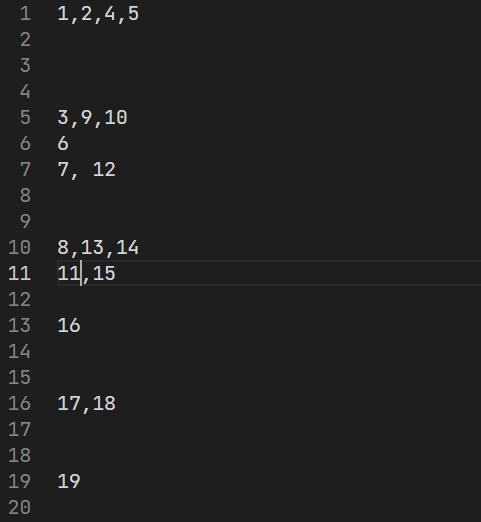
\includegraphics[width=\textwidth]{grafo_txt}
            \caption{Grafo adaptado en un archivo plano de texto.}
            \label{fig:grafo_txt}
        \end{figure}
        
        Observe el Listing \ref{lst:sistema_ups}, aquí simulamos la lectura del tomacorriente obteniendo números random. Por lo tanto en el momento en el que el voltaje se salga de los límites establecidos el UPS pasará al modo inversor y operará hasta que termine su ejecución. Puede ver su ejecución en la Figura \ref{fig:python_3} que se adapta al grafo de la Figura \ref{fig:grafo_cyber}.
        
        \lstinputlisting[
            language=Python,
            caption=Lectura de tomacorriente y gestion de UPS. Archivo System.py.,
            label=lst:sistema_ups,
            firstline=135,
            lastline=167
            ]{../../../src/System.py}
            
        \begin{figure}[H]
            \centering
            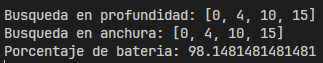
\includegraphics[width=\textwidth]{python_3}
            \caption{Grafo adaptado en un archivo plano de texto.}
            \label{fig:python_3}
        \end{figure}
            
            %%%%%%%%%%%%%%%%%%%%%%%%%%%%%%%%%%%%%%%%%%%%%%%%%%%%%%%%%%%%%%%%%
            %%                       DISCUSIÓN                             %%
    %%%%%%%%%%%%%%%%%%%%%%%%%%%%%%%%%%%%%%%%%%%%%%%%%%%%%%%%%%%%%%%%%
    \section{Discusión}
        % Aquí resuma brevemente sus hallazgos. En particular, la sección discusión proporcionará el significado, la importancia y la relevancia de los resultados de su trabajo. Al escribir la discusión del trabajo de investigación, debe concentrarse en proporcionar explicaciones y evaluar los hallazgos. Aquí usted puede incluir los hipervínculos de su video de presentación de su proyecto, así como el de su presentación.

        Se exploraron solo dos algoritmos de búsqueda por lo que el programa podría mejorar en ese aspecto. Además para conocer cual de los dos algoritmos empleados es mejor, sería idóneo hacer más pruebas con grafos mucho más grandes. Otra forma de determinar el mejor algoritmo es calcular su complejidad tanto espacial como temporal a través de librerías como \emph{Big O} de Python. Por otra parte resulta un poco confuso el uso de archivos para configurar el grafo, si bien es una alternativa rápida y simple para no tener que depender del todo del programa, si el programador o usuario que intente configurar desconozca por completa del tema, terminaría rompiendo el sistema.

        El UPS si bien cumple su función, se debe recordar que solo es una simulación del verdadero trabajo que realiza, así que los cálculos empleados pueden varíar en un escenario real. El sistema resulta algo incompleto en cuestión de mostrar todas las estadísticas del UPS, pero haría falta utilizar conceptos más avanzados como lo son hilos para usar el programa mientras simultaneamente se muestran dichas estadísticas. También cabe aclarar que el emplear un archivo donde se guarden los datos de las intensidades de cada uno de los dispositivos es por practicidad, dado que toda esa información sería directamente proporcionada por los sensores.

        Utilizar patrones de diseño resulta bastante útil ya que nos permite generalizar un programa y hacerlo flexible al cambio con el tiempo. Pero no siempre debe emplearse en todo momento ya que puede resultar contraproducente y terminar haciendo más complejo y abstracto el programa. No hay que forzar el uso de patrones, con la experiencia se puede identificar a simple vista cada uno de ellos, y es ahí donde es correcto emplearlos.

    %%%%%%%%%%%%%%%%%%%%%%%%%%%%%%%%%%%%%%%%%%%%%%%%%%%%%%%%%%%%%%%%%
    %%                       CONCLUSIONES                          %%
    %%%%%%%%%%%%%%%%%%%%%%%%%%%%%%%%%%%%%%%%%%%%%%%%%%%%%%%%%%%%%%%%%
    \section{Conclusiones}
        % La sección de conclusión debe reformular su teoría, resumir las ideas de apoyo clave que discutió a lo largo del trabajo y ofrecer su impresión final sobre la idea central. Este resumen final también debe contener la moraleja de su historia o una revelación de una verdad más profunda. Una buena conclusión resumirá sus pensamientos finales y puntos principales, combinando toda la información pertinente con un atractivo emocional para una declaración final que resuene con sus lectores.

        Dado la naturaleza de un circuito es mucho más complicado crear un grafo que sea bidireccional, por lo que la complejidad del problema no podría escalar demasiado en el escenario propuesto. Los grafos, si bien son una herramienta muy potente, no siempre puede aplicarse en todos los escenarios, pueden existir otras estructuras que den solución más rápidas o más livianas, en terminos de complejidad temporal. El objetivo siempre a la hora de encontrar una solución es buscar el equilibrio entre eficiencia y eficacia.

    %%%%%%%%%%%%%%%%%%%%%%%%%%%%%%%%%%%%%%%%%%%%%%%%%%%%%%%%%%%%%%%%%
    %%                       BIBLIOGRAFÍA                          %%
    %%%%%%%%%%%%%%%%%%%%%%%%%%%%%%%%%%%%%%%%%%%%%%%%%%%%%%%%%%%%%%%%%
    \nocite{*}
    \bibliographystyle{plain}
    \bibliography{bibliography}

\end{document}


% \lstinputlisting[
%     language=Python,
%     caption=Función de filtrado,
%     label=lst:filter_function,
%     firstline=208,
%     lastline=237
% ]{../../Python/src/Shop.py}